\renewcommand*{\arraystretch}{1.1}

\subsection*{Interactive / short / 7}
\label{section:interactive-short-read-07}

% change \emph{} to use sans-serif font
\let\oldemph\emph
\renewcommand{\emph}[1]{{\footnotesize \sf #1}}

\renewcommand{\currentQueryCard}{7}
\marginpar{
	\raggedleft
	\vspace{0.22ex}

	\queryRefCard{interactive-short-read-01}{IS}{1}\\
	\queryRefCard{interactive-short-read-02}{IS}{2}\\
	\queryRefCard{interactive-short-read-03}{IS}{3}\\
	\queryRefCard{interactive-short-read-04}{IS}{4}\\
	\queryRefCard{interactive-short-read-05}{IS}{5}\\
	\queryRefCard{interactive-short-read-06}{IS}{6}\\
	\queryRefCard{interactive-short-read-07}{IS}{7}\\
}


\noindent\begin{tabularx}{\queryCardWidth}{|>{\queryPropertyCell}p{\queryPropertyCellWidth}|X|}
	\hline
	query & Interactive / short / 7 \\ \hline
%
	title & Message Replies \\ \hline
%
	pattern & \multicolumn{1}{c|}{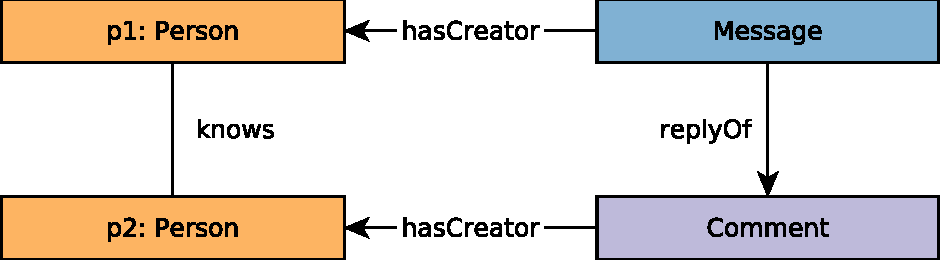
\includegraphics[scale=\patternscale,margin=0cm .2cm]{patterns/interactive-short-read-07}} \\ \hline
%
	desc. & Given a Message, retrieve the (1-hop) Comments that reply to it.

In addition, return a boolean flag \texttt{knows} indicating if the
author of the reply knows the author of the original message. If author
is same as original author, return false for \texttt{knows} flag.
 \\ \hline
%
	
		params &
		\innerCardVSpace{\begin{tabularx}{\attributeCardWidth}{|>{\paramNumberCell}c|>{\varNameCell}M|>{\typeCell}m{\typeWidth}|Y|} \hline
		$\mathsf{1}$ & Message.id
 & ID
 &  \\ \hline
		\end{tabularx}}\innerCardVSpace \\ \hline
	
%
	
		result &
		\innerCardVSpace{\begin{tabularx}{\attributeCardWidth}{|>{\resultNumberCell}c|>{\varNameCell}M|>{\typeCell}m{\typeWidth}|>{\resultOriginCell}c|Y|} \hline
		$\mathsf{1}$ & Message\textless{}-replyOf-Comment.id & ID & R &
				 \\ \hline
		$\mathsf{2}$ & Message\textless{}-replyOf-Comment.content & String & R &
				 \\ \hline
		$\mathsf{3}$ & Message\textless{}-replyOf-Comment.creationDate & DateTime & R &
				 \\ \hline
		$\mathsf{4}$ & Comment-hasCreator-\textgreater{}Person.id & ID & R &
				 \\ \hline
		$\mathsf{5}$ & Comment-hasCreator-\textgreater{}Person.firstName & String & R &
				 \\ \hline
		$\mathsf{6}$ & Comment-hasCreator-\textgreater{}Person.lastName & String & R &
				 \\ \hline
		$\mathsf{7}$ & knows & Boolean & C &
				Original message author knows reply author
 \\ \hline
		\end{tabularx}}\innerCardVSpace \\ \hline
	
%
	
		sort		&
		\innerCardVSpace{\begin{tabularx}{\attributeCardWidth}{|>{\sortNumberCell}c|>{\varNameCell}M|>{\directionCell}c|Y|} \hline
		$\mathsf{1}$ & Message\textless{}-replyOf-Comment.creationDate
 & $\desc
$ &  \\ \hline
		$\mathsf{2}$ & Message-hasCreator-\textgreater{}Person.id
 & $\asc
$ &  \\ \hline
		\end{tabularx}}\innerCardVSpace \\ \hline
	%
	%
	%
	%
\end{tabularx}
\queryCardVSpace

% change \emph back to the old one
\renewcommand{\emph}[1]{\oldemph{#1}}